\chapter{Third Party Tools and Resources}

\graphicspath{{../img/ch30/}}


In our solution we have exploited several tools and formalisms. These can be divided into two groups: linguistics and (inductive) logic programming. First we describe the linguistic tools and formalisms, the rest will follow.



\section{Prague Dependency Treebank (PDT)} \label{sec:ch30_pdt}
There exist several projects\footnote{Prague Dependency Treebank
 (PDT 1.0, PDT 2.0 \citep{biblio:PDT20_CD}), Prague English Dependency Treebank (PEDT 1.0), Prague Czech-English Dependency Treebank (PCEDT 1.0)} 
closely related to the ``Prague school of dependency linguistics’’ and the Institute of Formal and Applied Linguistics\footnote{\url{http://ufal.mff.cuni.cz}} in Prague, Czech Republic (ÚFAL). All the projects share common methodology and principles concerning the formal representation of natural language %(Czech above all; and recently also English)
 based on the theory of Functional Generative Description \citep{SgallHajicovaPanevova1986}.
We will refer to these principles and related formalism as ``PDT principles and formalisms’’ in the present work because the PDT projects are the most fundamental and the elaborate annotation guidelines (see bellow) were compiled within these projects. The most relevant principles for the present work will be briefly described in this section.

\subsection{Layers of Dependency Analysis in PDT}

Unlike the usual approaches to the description of English syntax, the Czech syntactic descriptions are dependency-based, which means that every edge of a syntactic tree captures the relation of dependency between a governor and its dependent node. 

In PDT, text is split into individual sentences and dependency trees are built form them. Nodes of the trees are represented by individual words or tokens and edges represent their linguistic dependencies (simplified speaking, see bellow). Among others, two most important kinds of dependencies are distinguished: syntactical dependencies and ``underlying (deep) structure’’ dependencies. Syntactical dependencies are often called \emph{analytical} and the latter are called \emph{tectogrammatical} dependencies. These two kinds of dependencies form two kinds of dependency trees: \emph{analytical trees} and \emph{tectogrammatical trees}. The situation is usually described using a concept of different layers (or levels) of annotation. It is illustrated by Figure~\ref{fig:ch30_layers}. The description starts at the bottom with the surface structure of a sentence (\emph{w-layer}); note that there is a spelling error -- missing space between words `do’ and `lesa’ (into forest) in the example sentence. The lowest level of linguistic annotation (\emph{m-layer}) represents morphology. Word forms are disambiguated and correct lemmas (dictionary form) and morphological tags are assigned at this level. The second level of annotation is called analytical (\emph{a-layer}). At this level the syntactical dependencies of words are captured (e.g. subject, predicate, object, attribute, adverbial, etc.) The top level of annotation is called tectogrammatical (\emph{t-layer}), sometimes also called ``layer of deep syntax''. At this level some tokens (e.g. tokens without lexical meaning) are leaved out or ``merged’’ together (e.g. prepositions are merged with their ``targets’’). Also some nodes without a morphological level counterpart are inserted to the tectogrammatical tree at certain occasions (e.g. a node representing omitted subject -- on Figure~\ref{fig:ch30_layers} labeled as ``\#PersPron’’).  

More over all the layers of PDT sentence representation are interconnected and additional linguistic features are assigned to tree nodes. Among others: \emph{morphological tag} and \emph{lemma} is assigned at the morphological level; \emph{analytical function} (the actual kind of the particular analytical dependency, e.g. predicate, subject, object, etc.) is assigned to dependent nodes at the analytical level; \emph{semantic parts of speech} + \emph{grammatemes} (e.g. \emph{definite quantificational semantic noun} (n.quant.def) + \emph{number} and \emph{gender}, etc.) and \emph{tectogrammatical functor} (e.g. actor (ACT), patient (PAT), addressee (ADDR), temporal: when (TWHEN), directional: to (DIR3), etc.) is assigned at the tectogrammatical level. 

\medskip
Detailed information can be found:
\begin{itemize}
	\item Homepage of the PDT 2.0 project: \url{http://ufal.mff.cuni.cz/pdt2.0/}
	\item Annotation guidelines:	
	\begin{itemize}
		\item Morphological Layer Annotation \citep{mmanCz2005}
		\item Analytical Layer Annotation \citep{amanEn1999}
		\item Tectogrammatical Layer Annotation \citep{biblio:MiBeAnnotationtectogrammatical2006}
		\item Tectogrammatical Layer Annotation for English (PEDT 1.0) \citep{biblio:CiHaAnnotationEnglish2006}
		
	\end{itemize}	
\end{itemize}

\subsection{Why Tectogrammatical Dependencies?}

The practice has shown that representing only syntactical roles of tokens present in a sentence is not sufficient to capture the actual meaning of the sentence. Therefore the tectogrammatical level of representation was established.

Or according to \cite{biblio:KlTransformationBasedTectogrammatical2006}:

\begin{quote}
Annotation of a sentence at this [tectogrammatical] layer is closer to meaning of the sentence than its syntactic annotation and thus information captured at the tectogrammatical layer is crucial for machine understanding of a natural language. This can be used in areas such as machine translation and information retrieval, however it can help other tasks as well, e.g. text synthesis.	
\end{quote}


\begin{figure}
	\begin{center}
	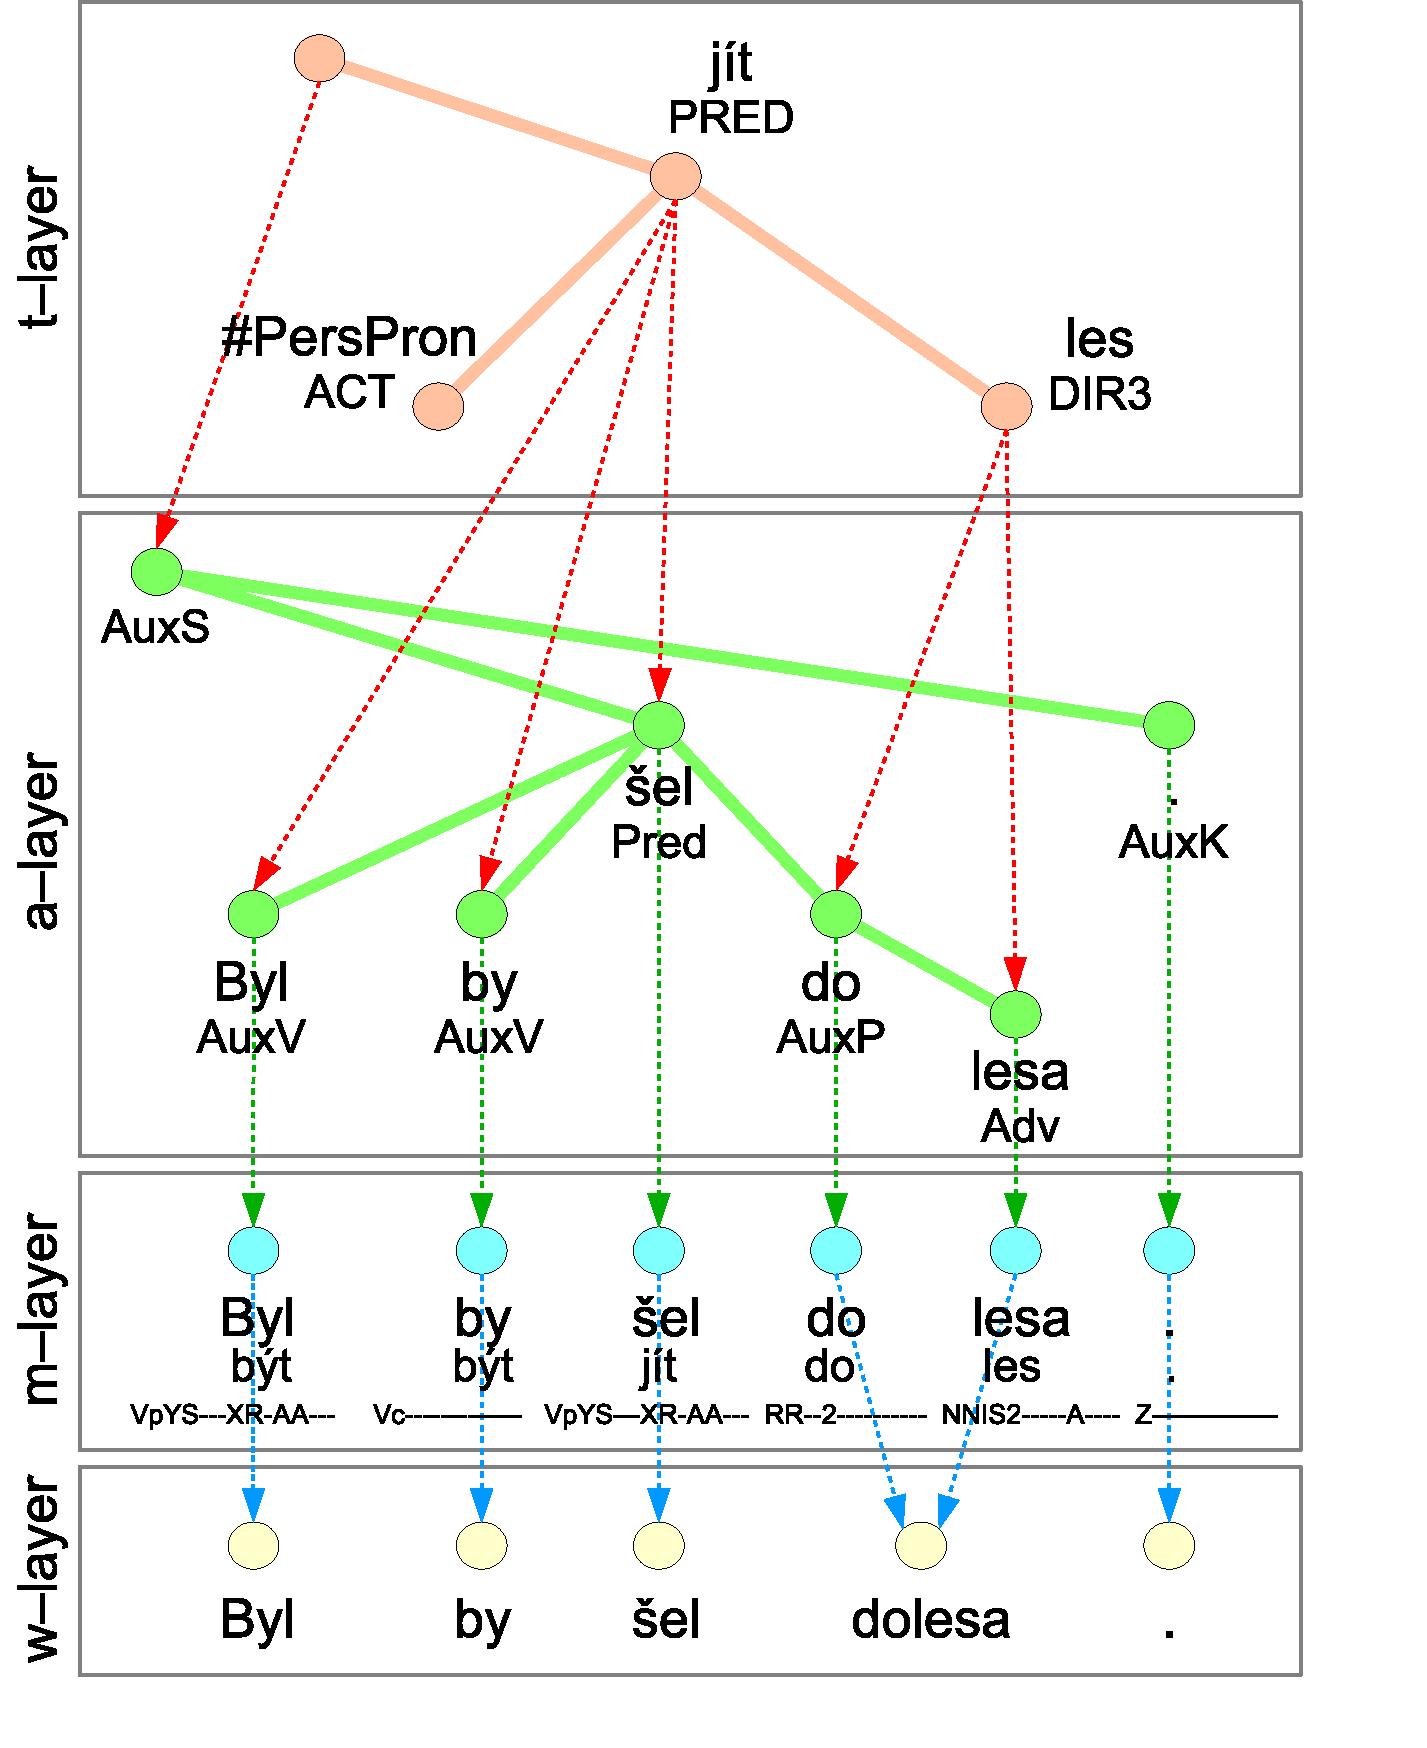
\includegraphics[width=0.6\hsize]{PDT_layers}
		\begin{tabular}{rlllll}
Sample sentence (in Czech): & & Byl & by & šel & dolesa.\\
English translation (lit.):& [He] & would & have & gone & intoforest.			
		\end{tabular}
	\end{center}
\caption{Layers of linguistic annotation in PDT}
\label{fig:ch30_layers}
\end{figure}





\section{PDT Tools and Resources} \label{sec:ch30_pdt_tools_and_resources}

In this section several linguistic tools and resources that are being developed at ÚFAL will be described. These tools and resources are closely connected with the PDT projects and they have been used also in the present work for various purposes.


%%%%%%%%%%%%%%%%%%%%%%%%%%%%%%%%%%%%%%%%%%%%%%%%%%%%%%%%%%%%%%%%%%%%%%%%%%%%%%%%%%%%%%%%%%%%%%%%%
\subsection{Linguistics Analysis} \label{sec:ch30_ling_tools}
%%%%%%%%%%%%%%%%%%%%%%%%%%%%%%%%%%%%%%%%%%%%%%%%%%%%%%%%%%%%%%%%%%%%%%%%%%%%%%%%%%%%%%%%%%%%%%%%%

Linguistic tools that were used for automated (machine) linguistic annotations of texts will be briefly described in this section. These tools are used as a processing chain and at the end of the chain they produce tectogrammatical dependency trees. 


 
\subsubsection{Tokenization and Segmentation} 
On the beginning of text analysis the input text is divided into tokens (words and punctuation); this is called \emph{tokenization}. Sequences of tokens are then (or simultaneously) divided into sentences; this is called \emph{segmentation}. Note that although the task seems quite simple, especially segmentation is not trivial and painful errors occur at this early stage e.g. caused by abbreviations ended by full stop in the middle of a sentence.

There are several tools available for Czech and English. The oldest (Czech) one can be found on the PDT 2.0 CD-ROM \cite{biblio:PDT20_CD} and several choices are provided by TectoMT (see Section~\ref{sec:ch30_tectomt}) and GATE (see Section~\ref{sec:ch30_gate}). The best choice for Czech is probably TextSeg \citep{TextSeg}, which is available through TectoMT.


		
\subsubsection{Morphological Analysis}

Because Czech is a language with rich inflections, morphological analysis (or at least lemmatization) is an important means to success of any NLP task (starting with key word search and indexing.) In PDT morphological analysis is a necessary precondition for analytical analysis (next section).

The task of morphological analysis is for given word form in given context to select the right pair of lemma (dictionary form) and morphological tag. In PDT the tag includes part of speech (POS) and other linguistic categories like gender, number, grammatical case, tense, etc., see morphological annotation guidelines for details.

For Czech two main tools are available: Feature-based tagger\footnote{\url{http://ufal.mff.cuni.cz/tools.html/fbtag.html}} by \cite{biblio:HajicMorfTag} and perceptron-based tagger Morče\footnote{\url{http://ufal.mff.cuni.cz/morce/}} by \cite{biblio:VoMorphologicalTagging2006}. Morče is several years newer and it achieved few points better accuracy on PDT 2.0 (94.04\% vs. 95.12\% see in \citep{Spoustova07b}). Both tools are available through TectoMT, Morče also for English.

\subsubsection{Analytical Analysis}

The task of Analytical analysis is to build up a syntactical dependency tree (analytical tree) from a morphologically analyzed sentence and to assign right kind of dependency (analytical function) to every edge of the tree.


There were experiments with almost all well known parsers on the Czech PDT data\footnote{See details at \url{http://ufal.mff.cuni.cz/czech-parsing/}}. But two of them have proved in practice: Czech adaptation of Collins' parser \citep{biblio:collinshbrt_1999} and Czech adaptation of McDonald's MST parser \citep{Novak:2007:FEM:1776334.1776350}. Again the second tool is few years newer and few points better in accuracy (80.9\% vs. 84.7\% on PDT 2.0\footnotemark[\value{footnote}]). The Collins' parser can be found on the PDT 2.0 CD-ROM and the MST parser is available through TectoMT.

The analytical analysis of English is not very well established because PEDT 1.0\footnote{\url{http://ufal.mff.cuni.cz/pedt/}} contains only tectogrammatical level of annotation and there is no other English treebank for the analytical level. The English analytical analysis is regarded rather as a part of English tectogrammatical analysis; see details in \citep{Klimes:2007:TTD:1776334.1776341}.



%\textbf{Analytical function assignment} \citep{biblio:AlyticAsign} assigns a description (\emph{analytical function}, in linguistic sense) to every edge in the syntactic (dependency) tree.
	
\subsubsection{Tectogrammatical Analysis}

During tectogrammatical analysis analytical trees are transformed to tectogrammatical ones. Merging, omitting and inserting of tree nodes takes place as well as assignment of all the complex linguistic information of the tectogrammatical level (semantic parts of speech, grammatemes, tectogrammatical functors, etc.)

The tectogrammatical analysis can by performed by a variety of TectoMT ``blocks'' (depending on the amount of requested linguistic information, for example only tectogrammatical functors can be assigned.) Better results can be obtained through transformation-based tools developed by Václav Klimeš: \citep{biblio:KlTransformationBasedTectogrammatical2006} for Czech and \citep{Klimes:2007:TTD:1776334.1776341} for English; they are also available thorough TectoMT.


%\begin{table}
%\centering
	%\begin{tabular}{l|l}
		%Name of the tool & Evaluation results (proclaimed by authors) \\[4pt]
		%\hline
	%Segmentation and tokenization & precision(p): 98,0\%, recall(r): 91,4\% \\[4pt]
	%Morphological analysis & 2,5\% unrecognized words\\
	%Morphological tagging & 93,0\% of tags assigned correctly \\[4pt]
	%Collins' parser -- Czech adaptation & 81,6\% dependencies assigned correctly\\
	%Analytical function assignment & precision: 92\% \\[4pt]
	%Tectogrammatical analysis & dependencies p:~90,2\%, r:~87,9\%\\
	%& assignment of f-tags p:~86,5\%, r:~84,3\%\\
	%\end{tabular}
%\caption{Linguistic tools for machine annotation}
%\label{tab:ling_tools}
%\end{table}
%

\subsection{Tree Editor TrEd, Btred}

TrEd is the ÚFAL key tool for work with dependency based linguistic annotations. It provides a comfortable GUI for navigation, viewing and editing of linguistic trees at different levels of annotation, for different languages and different treebank schemas. TrEd is implemented in Perl and it is available for a variety of platforms (Windows, Unix, Linux, Mac OS X).

\medskip
Homepage of the project: \url{http://ufal.mff.cuni.cz/~pajas/tred/}


\subsubsection{Btred}
TrEd can be also controlled using a powerful set of Perl macros and there is also a non-interactive version of TrEd called Btred, which allows batch evaluation of user macros on an arbitrary set of annotated documents.

\medskip
Btred/ntred tutorial: \url{http://ufal.mff.cuni.cz/~pajas/tred/bn-tutorial.html}


\subsubsection{PML Tree Query} \label{sec:ch30_pml_tree_query}
PML Tree Query (PML-TQ) \citep{biblio:PaStSystemfor2009} is a TrEd based module for searching through a treebank using a complex tree based query language.

\medskip
Homepage of the project: \url{http://ufal.mff.cuni.cz/~pajas/pmltq/}



\subsection{TectoMT} \label{sec:ch30_tectomt}
%As we have started with our native language -- Czech (a language with rich morphology and free word order), we had to make tools for processing Czech available in GATE. We have implemented a wrapper for the TectoMT system\footnote{\url{http://ufal.mff.cuni.cz/tectomt/}}  to GATE.

TectoMT \citep{biblio:ZaPtTectoMTHighly2008} is a Czech project that contains many linguistic tools for different languages including Czech and English; all the tools are based on the dependency based linguistic theory and formalism of PDT. It is implemented in Perl; highly exploiting TrEd libraries. The recommended platform is Linux. %Windows (not recomended platform for TectoMT)
It is primarily aimed at machine translation but it can also facilitate development of software solutions of other NLP tasks.

We have used a majority of applicable tools from TectoMT (e.g. tokeniser, sentence splitter, morphological, analytical and tectogrammatical analyzers for Czech and English). We have also developed TectoMT wrapper for GATE, which makes it possible to use TectoMT tools inside GATE, see details in Section~\ref{sec:ch60_tectomt_wrapper}.

Similarly to GATE, TectoMT supports building of application pipelines (\emph{scenarios}) composed of so called \emph{blocks} -- processing units responsible for single independent task (like tokenization, parsing, etc.)

\medskip
Homepage of the project: \url{http://ufal.mff.cuni.cz/tectomt/}


\subsection{Netgraph} \label{sec:ch30_netgraph}

Netgraph \citep{biblio:MiNetgraphA2006} is a linguistic tool used for searching through a syntactically annotated corpus of a natural language (corpus of linguistic dependency trees). Besides the searching capabilities it also provides a GUI for viewing of dependency trees. Both of these features were exploited in the present work.

Netgraph implementation is client-server based and a special query language is used for searching. The query language allows putting restrictions on the shape of a tree and on values of attributes of an arbitrary tree node. Besides that nodes of a query can be marked as optional (not necessarily present in a matching tree) and names can be assigned to query nodes. Naming of query nodes then allows putting restrictions based on referenced nodes (Give me all trees where there is a node with two children and both children have the same lemma.) See also Section~\ref{sec:ch50_Netgraph_Based_Extraction_Rules}, it provides additional information about the query language including example Netgraph queries.

Currently Netgraph is replaced by PML Tree Query (see Section~\ref{sec:ch30_pml_tree_query}) and the Netgraph development is ``discontinued''. We use Netgraph in the present work because it is written in Java, the language of what we use. This also made it possible to use Netgraph inside GATE as a handy viewer of dependency trees, see Section~\ref{sec:ch60_GATE_Netgraph}. 

\medskip
Homepage of the project: \url{http://quest.ms.mff.cuni.cz/netgraph/}


\subsection{Annotation Schemas}
\subsubsection{Prague Markup Language (PML)} \label{sec:ch30_pml}
\subsubsection{Feature Structure (FS)} \label{sec:ch30_fs}


\section{Czech WordNet}

The Figure~99 shows, that it would be useful to gather words with similar meanings in our extraction rules. For example, the rule in the Figure~99 contains long disjunctions of similar words (nodes with numbers 1 and 4). These disjunctions could be replaced with some kind of expression telling that we are looking for any word from some semantic category (e.g. human beings). For this purpose we wanted to use the Czech WordNet \citep{biblio:WordNetCZ2004}. 

After we have explored the records of the Czech WordNet (CzWN) related to the domain of our interest (car accidents, etc.) we have decided not to involve CzWN in the extraction process. The reason is that the coverage of the vocabulary of our domain is rather poor and the semantic connections of words are sometimes unfortunately missing. But we can supply the missing information to CzWN or we can build up a new domain-specific word-net based on the ground of CzWN.  

\medskip
Availability: \url{http://catalog.elra.info/product_info.php?products_id=1089}



\section{GATE} \label{sec:ch30_gate}
GATE \citep{biblio:GATE_ACL2002} is probably the most widely used tool for text processing. In our solution the capabilities of document and annotation management, utility resources for annotation processing, JAPE grammar rules \citep{Cunningham00jape:a}, machine learning facilities and performance evaluation tools are the most helpful features of GATE that we have used.

\medskip
Homepage of the project: \url{http://gate.ac.uk/}

\subsection{GATE Annotations} \label{sec:ch30_gate_annotations}
Contrary to PDT, GATE annotations\footnote{\url{http://gate.ac.uk/userguide/sec:corpora:dags}} are rather simple and minimalistic. They are designed as labeled segments of text. A single annotation is described by its label (\emph{annotation type}) and starting and ending character offset. Each annotation has a unique identifier (integer ID) and an arbitrary set of \emph{features}\footnote{\url{http://gate.ac.uk/userguide/sec:corpora:features}} (name-value pairs) can be assigned to it. 

For example in a sentence ``Hamish Cunningham leads the GATE team.'', ``Hamish Cunningham'' can be annotated with a GATE annotation starting at character 0, ending at character 16, annotation type: ``Person'', with three features: ``firstName=Hamish; surname= Cunningham; gender=male''; because it is the only annotation, the ID would most probably be 0.

Although the GATE annotation approach seems quite simple, very complex structures can be encoded this way (for example an annotation feature can contain a reference to another annotation using its ID), but such usage of GATE annotations is always tricky to some degree and it is always necessary to establish a convention about that. In Section~\ref{sec:ch60_pdt_in_gate} encoding of PDT dependency annotations in GATE will be presented.


%%%%%%%%%%%%%%%%%%%%%%%%%%%%%%%%%%%%%%%%%%%%%%%%%%%%%%%%%%%%%%%%%%%%%%%%%%%%%%%%%%%%%%%%%%%%%%%%%
\section{Named Entity Recognition} \label{sec:ch30_named_entity_recognition}
%%%%%%%%%%%%%%%%%%%%%%%%%%%%%%%%%%%%%%%%%%%%%%%%%%%%%%%%%%%%%%%%%%%%%%%%%%%%%%%%%%%%%%%%%%%%%%%%%


%%%%%%%%%%%%%%%%%%%%%%%%%%%%%%%%%%%%%%%%%%%%%%%%%%%%%%%%%%%%%%%%%%%%%%%%%%%%%%%%%%%%%%%%%%%%%%%%%
\section{Inductive Logic Programming} \label{sec:ch30_ILP}
%%%%%%%%%%%%%%%%%%%%%%%%%%%%%%%%%%%%%%%%%%%%%%%%%%%%%%%%%%%%%%%%%%%%%%%%%%%%%%%%%%%%%%%%%%%%%%%%%

Inductive Logic Programming (ILP) \citep{biblio:MuggletonILP} is a machine learning technique based on logic programming. Given an encoding of the known background knowledge (in our case linguistic structure of all sentences) and a set of examples represented as a logical database of facts (in our case tokens annotated with the target annotation type are positive examples and the remaining tokens negative ones), an ILP system will derive a hypothesized logic program (in our case extraction rules) which entails all the positive and none of the negative examples.

Formal definitions of ILP tasks are presented in following sections. They will be extended and used for implementation of Fuzzy ILP Classifier in Chapter~\ref{sec:ch80_fuzzy_ilp_chapter}.






%To make the text easier to read, we present a short description of the ILP techniques below.

%%%%%%%%%%%%%%%%%%%%%%%%%%%%%%%%%%%%%%%%%%%%%%%%%%%%%%%%%%%%%%%%%%%%%%%%%%%%%%%%%%%%%%%%%%%%%%%%%
\subsection{Classical ILP} \label{sec:ch30_ILP_classic}
%%%%%%%%%%%%%%%%%%%%%%%%%%%%%%%%%%%%%%%%%%%%%%%%%%%%%%%%%%%%%%%%%%%%%%%%%%%%%%%%%%%%%%%%%%%%%%%%%

In our presentation of ILP we follow \cite{dzeroski2001:relat_dm} and  \cite{biblio:Muggleton94inductivelogic}.


\theoremstyle{definition}
\newtheorem{definition}{Definition}
\newtheorem{theorem}{Theorem}

\begin{definition}[Classical ILP task]
A set of examples $E=P\cup N$, where $P$ contains positive and $N$ negative examples, and background knowledge denoted by $B$ are given. The task of ILP is to find a hypothesis $H$ such that 

$$
(\forall e\in P)(B\cup H\models e)
$$
and
$$
(\forall e\in N)(B\cup H\not\models e).
$$
\end{definition}
Typically, $E$ consists of ground instances of the target predicate, in our case tree nodes relevant for the praticular extraction task or accident seriousness (see examples in Figure~\ref{img:examples}). $B$ typically consists of several predicates (relational tables), which describe properties of an object, in our case properties of an accident (see examples in Figure~\ref{img:crisp_attributes}) or the structure and properties of linguistic trees. The background knowledge can also contain some rules. A hypothesis $H$ typically consists of logic programming rules (see examples in Figure~\ref{img:rules} and Figure~\ref{fig:rules}). $H$ added to $B$ entails all positive examples and no negative examples.
%
The main advantage of ILP is its multirelational character, namely, $B$ can reside in several relational tables.





%%%%%%%%%%%%%%%%%%%%%%%%%%%%%%%%%%%%%%%%%%%%%%%%%%%%%%%%%%%%%%%%%%%%%%%%%%%%%%%%%%%%%%%%%%%%%%%%%
\subsection{Fuzzy ILP}
%%%%%%%%%%%%%%%%%%%%%%%%%%%%%%%%%%%%%%%%%%%%%%%%%%%%%%%%%%%%%%%%%%%%%%%%%%%%%%%%%%%%%%%%%%%%%%%%%

In our presentation of fuzzy ILP we follow the paper of 
%T. Horv\'ath and P. Vojt\'a\v s 
\cite{biblio:FILP} about fuzzy inductive logic programming.
We use the approach of the fuzzy logic in a narrow sense, developed by 
%J.~Pavelka
\cite{biblio:Pavelka} and 
%P. H\'ajek 
\cite{biblio:Hajek}. Formulas are of the form $\varphi, x$ ($\varphi$ is syntactically the same as in the classical case), they are graded by a truth value $x\in [0,1]$.
A structure ${\mathcal M}$ consists of a domain $M$ and relations are interpreted as fuzzy (we do not consider function symbols here). The evaluation $\left\|\varphi\right\|_{{\mathcal M}}$ of a formula $\varphi$ uses truth functions of many-valued connectives (our logic is extensional and/or truth functional). The satisfaction $\models_f$ is defined by
$$
{\mathcal M}\models_f (\varphi, x)\ iff\ \left\|\varphi\right\|_{{\mathcal M}}\ge x.
$$

\begin{definition}[Fuzzy ILP task]
A fuzzy set of examples ${\mathcal E}:E\longrightarrow [0,1]$ and a fuzzy background knowledge ${\mathcal B}:B\longrightarrow [0,1]$ are given. The task of fuzzy ILP is to find a fuzzy hypothesis ${\mathcal H}:H\longrightarrow [0,1]$ such that 

$$
(\forall e_1,e_2\in E)(\forall {\mathcal M})({\mathcal M}\models_f {\mathcal B}\cup {\mathcal H})
$$
we have
$$
{\mathcal E}(e_1)>{\mathcal E}(e_2)\Rightarrow \left\|e_1\right\|_{{\mathcal M}}\ge \left\|e_2\right\|_{{\mathcal M}}.
$$
That is, it cannot happen that
$$
{\mathcal E}(e_1)>{\mathcal E}(e_2) \wedge \left\|e_1\right\|_{{\mathcal M}}< \left\|e_2\right\|_{{\mathcal M}},
$$
or rephrased: if ${\mathcal E}$ is rating $e_1$ higher than $e_2$, then it cannot happen that $e_1$ is rated worse than $e_2$ in a model of ${\mathcal B}\cup {\mathcal H}$.
\end{definition}

Typically, ${\mathcal E}$ consists of ground instances of the target predicate, which are classified in truth degrees, in case of accident classification, degrees of seriousness of an accident. ${\mathcal B}$ typically consists of several fuzzy predicates (fuzzy relational tables), which describe properties of an object, in our case fuzzy properties of an accident -- a degree of injury, a degree of damage, etc. 
%Background knowledge can contain also some rules, so far only crisp rules are used.
A~hypothesis ${\mathcal H}$ typically consists of a fuzzy logic program, which, when added to ${\mathcal B}$, prevents misclassification (what is better cannot be declared to be worse, nevertheless it can be declared as having the same degree -- for more detailed discussion on this definition of fuzzy ILP we refer to the paper \citep{biblio:FILP}).


\subsection{ILP tool} \label{sec:ch30_ILP_tool}
As an ILP tool we have used ``A Learning Engine for Proposing Hypotheses'' (Aleph v5)\footnote{\url{http://www.comlab.ox.ac.uk/activities/machinelearning/Aleph/}}, which we consider very practical. It uses quite effective method of inverse entailment \citep{biblio:InverseEntailment} and keeps all handy features of a Prolog system (we have used YAP Prolog\footnote{\url{http://www.dcc.fc.up.pt/~vsc/Yap/}}) in its background.


Na rozdil od prologu examples we dvou souborech.

\medskip
Homepage of the project: \url{http://www.comlab.ox.ac.uk/activities/machinelearning/Aleph/}



From our experiments (Section~\ref{sec:evaluation}) can be seen that ILP is capable to find complex and meaningful rules that cover the intended information.



\textbf{?? large amount of training data ??}

As we do not have large amount of training data, there is no problem with excessive time demands during learning and the application of the learned rules is simple and quick.



\section{Weka} \label{sec:ch30_weka}

Weka \citep{biblio:Weka} is a well known data-mining software.

Weka data mining software\footnote{\url{http://www.cs.waikato.ac.nz/ml/weka/}} \citep{biblio:Weka}

Weka Experimenter 

experimenter

usage: evaluation of Fuzzy ILP Classifier (Section~\ref{sec:ch80_eval})

\medskip
Homepage of the project: \url{http://www.cs.waikato.ac.nz/ml/weka/}

